
	
\section{Progettazione a fatica}
\subsection{Curva classica di Wöhler}
			La classica cura di Wöhler si ottiene in condizioni di probabilità di rottura fissata e per rapporto di ciclo pari a -1 e con $\sigma_m$ nulla. \newline
			
			Come si ricava la pendenza del diagramma di Wöhler? 
\begin{figure}[H]
	\centering
	\label{fig:screenshot002}
	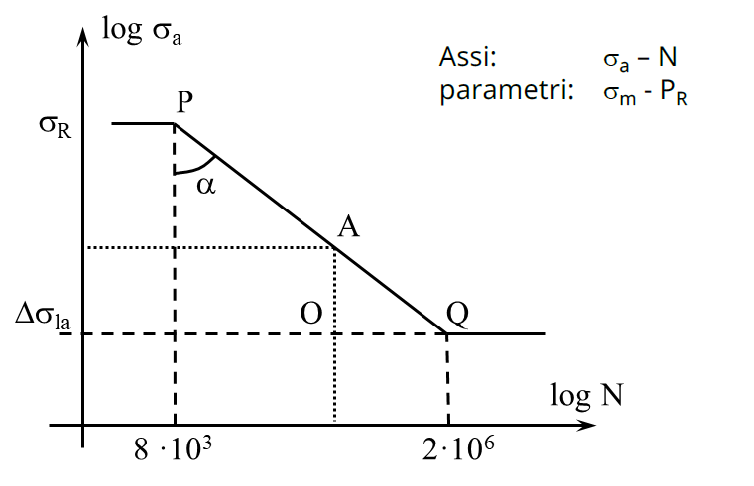
\includegraphics[width=0.5\linewidth]{immagini_11/screenshot002}
\end{figure}
			$k$ è l'inverso della pendenza, nel diagramma doppio-logaritmico questa è legata all'anglo $\alpha$, tuttavia la pendenza solitamente è espressa come $\dfrac{\Delta y}{\Delta x}$ ovvero come il complementare ad $\alpha$. 
			
			La tangente di $\alpha$ è data da $\dfrac{\Delta x}{\Delta y}$, se si immagina di conoscere la coppia di valori limite relativa al punto $A$ sul diagramma di Wöhler, e avendo dalla teoria noti i valori di $P, Q$, per ricavare la pendenza si può porre:
			\[\tan\alpha = \dfrac{\bar{QO}}{\bar{AO}} = \dfrac{\log N_Q - \log N_A}{\log\sigma_A - \log\sigma_Q} = k\]
			Per cui:
			\[\log\left(\dfrac{N_Q}{N_A}\right) = k\log\left(\dfrac{\sigma_A}{\sigma_Q}\right)\]
			E quindi:
			\[N_Q\sigma_Q^k = N_A\sigma_A^k = N\sigma^k = \, \text{cost}\]
			Maggiore è $k$ e meno pendente risulterà il diagramma. \newline 
			
			Questo vuol dire che siccome $P$ è fissato dal materiale, ovvero dalla sua rottura, una $k$ più grande e quindi una curva meno pendente vuol dire un provino che dura di più: si incontra la curva molto più tardi. \newline 
			
			I valori indicativi di $k$ sono intorno a 8$\div$10 per provini lisci, mentre in presenza di intagli si aggirano intorno ai 3$\div$6. \newline
			
			Si ricorda che il ginocchio non è "presente" per i materiali che non hanno ferro all'interno viene lo stesso preso convenzionalmente a $10^8$ cicli. 
			
\section{Altri diagrammi di fatica}			
			Il classico diagramma di Wöhler è rappresentato per tensioni medie nulle, se si vanno a diagrammare casi con $\sigma_m\ne0$ si trovano curve che si abbassano a parità di tensione massima, questo perché aumentando la sigma media deve ridursi la semiampiezza: al crescere della sigma media si riscontra una riduzione del diagramma, tuttavia non è possibile sapere l'entità della riduzione dato che  il diagramma di Wöhler non ne fornisce l'informazione. \newline 
			
			Per rappresentare una condizione limite di fatica bisogna identificare quattro parametri: o $\sigma_m$, $\Delta\sigma$ o in alternativa $\sigma_{\max}$ e $\sigma_{\min}$ oppure ancora $N$ e $P_R\%$. 
			
			Quest'ultimo termine (la probabilità di rottura) può mantenersi bloccato: si ottengono semplicemente diagrammi scalati in funzione della rappresentazione probabilistica di cui si necessita. 
			
			I restanti parametri si possono così combinare a due a due per avere diverse rappresentazioni della condizione critica. \newline 
			
			Come ampiamente detto il diagramma di Wöhler fissava la $\sigma_m$ e usava semiampiezza $\Delta \sigma$ ed $N$. 
			
			Una rappresentazione diversa, quella di Haig prevede che su le ascisse si metta la $\sigma_m$ e sulle ordinate la $\Delta \sigma$, a fissati $N$.
			\begin{figure}[H]
				\centering
				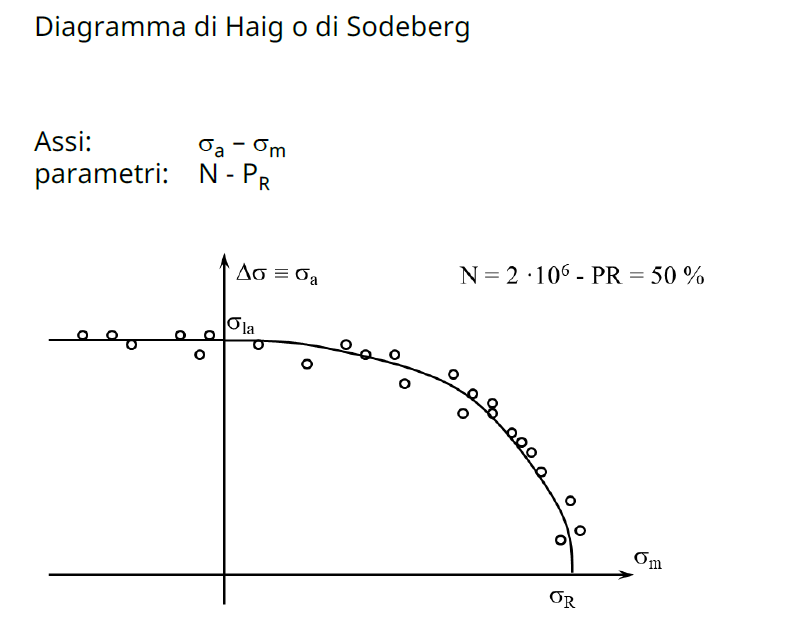
\includegraphics[width=0.5\linewidth]{immagini_11/screenshot003}
				\label{fig:screenshot003}
			\end{figure}			
			Standardizzando l'operazione, i cicli che si possono fissare sono quelli del ginocchio di Wöhler $10^6$ si vanno poi a riportare su questo diagramma tutti quei provini che si sono rotti applicando $10^6$ volte il carico: la popolazione di provini rotti a questo ciclo di sollecitazione si distribuisce secondo questa funzione, una sorta di parabola nel primo quadrante con un andamento lineare nel secondo. \newline
			
			Quando siamo a $\sigma_R$ che condizione sto caricando? $\sigma_m, \Delta\sigma\ne0$, ma com'è lo spettro di carico a semiampiezza nulla? Costante.
			
			Questa è la condizione critica statica: è stato applicato $\sigma_R$ (il carico di rottura) quando sono a $\sigma_{la}$ invece cosa ho? Sollecitazione alterno simmetrica a sigma media nulla, quello è il valore di semiampiezza del ginocchio della cura di Wöhler standard: era la semiampiezza a $10^6$ cicli valutata per una sigma media nulla. 
			
			Altre combinazioni intermedie si distribuiscono lungo un ramo di parabola, le sigma medie di compressione sono nel secondo quadrante (favorevoli), mentre la semiampiezza limite rimane constante. \newline 
			 
			Tale curva può essere rappresentata mediante la parabola di Gerber.
			\begin{figure}[H]
				\centering
				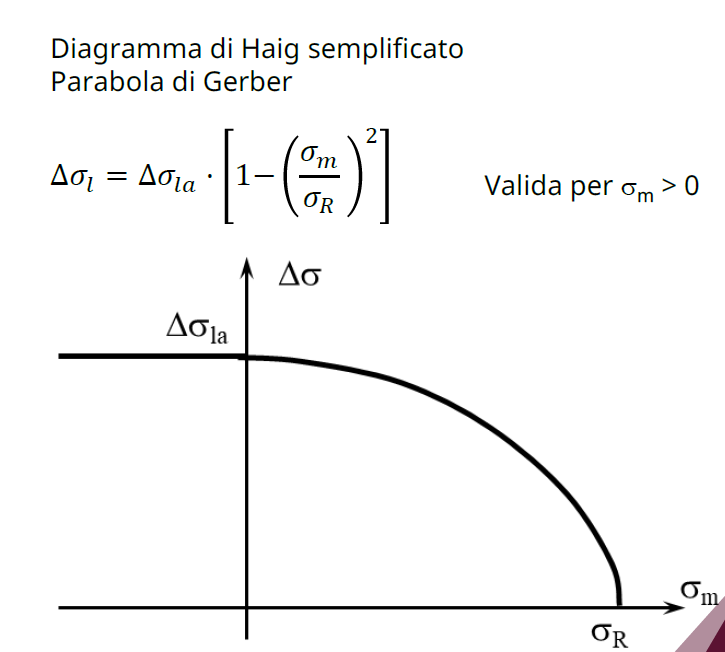
\includegraphics[width=0.5\linewidth]{immagini_11/screenshot004}
				\label{fig:screenshot004}
			\end{figure}			 
			Poiché ci si vuole mantenere in condizioni di sicurezza, la parabola di Gerber viene approssimata da Goodman come una semplice retta che passi per la condizione alterno simmetrica standard e per quella statica. 
			\begin{figure}[H]
				\centering
				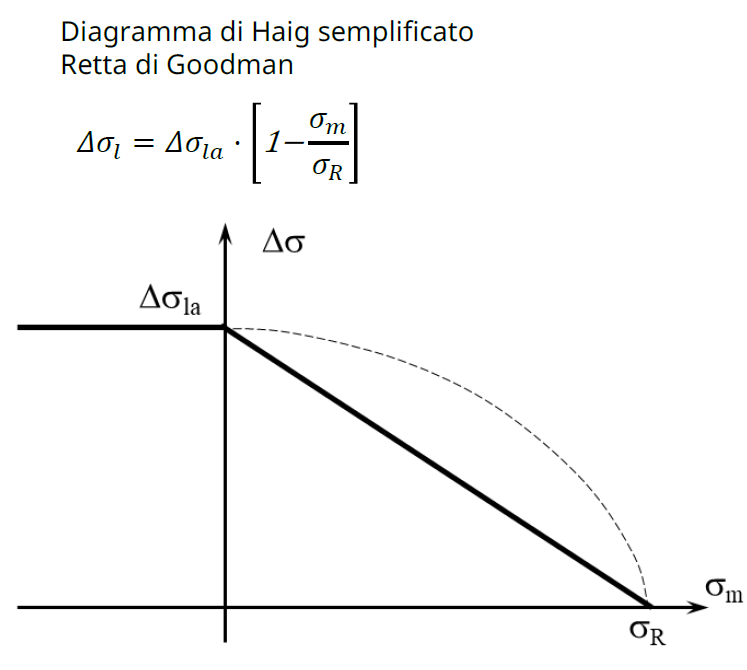
\includegraphics[width=0.5\linewidth]{immagini_11/screenshot005}
				\label{fig:screenshot005}
			\end{figure}						
			A causa della duttilità di alcuni materiali non è preferibile avere una condizione limite a rottura, allora Soderberg considera approssimabile e correggibile questa retta con un limite statico allo snervamento, semplicemente spostando, abbassando la curva che ora passa per $\sigma_Y$ anziché $\sigma_R$.
			\begin{figure}[H]
				\centering
				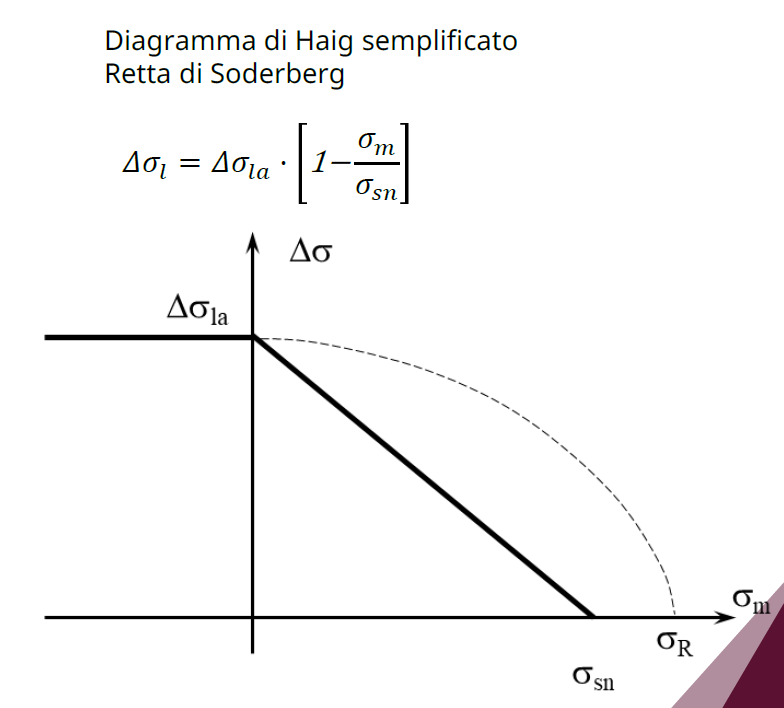
\includegraphics[width=0.5\linewidth]{immagini_11/screenshot006}
				\label{fig:screenshot006}
			\end{figure}
			Questa curva tuttavia risulta troppo conservativa rispetto ai dati sperimentali, questi appartenenti alla parabola iniziale, per i materiali duttili si utilizza allora una rappresentazione semplificata: la curva di Goodman viene corretta localmente attraverso una spezzata sia a trazione che a compressione che punta alle rispettive condizioni di snervamento statico, insieme alla condizione alternata che punta anch'essa allo snervamento
			\begin{figure}[H]
				\centering
				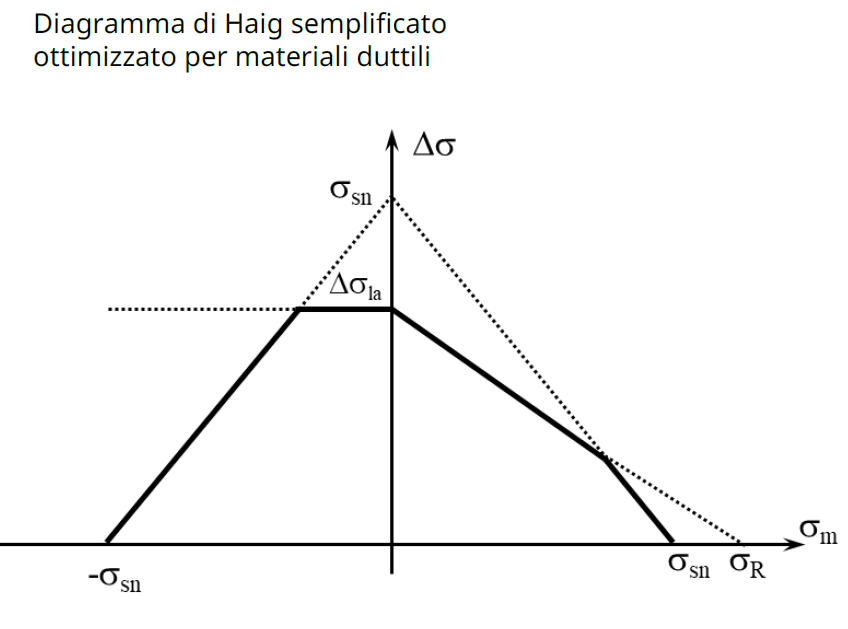
\includegraphics[width=0.5\linewidth]{immagini_11/screenshot007}
				\label{fig:screenshot007}
			\end{figure}			
			È possibile in questo modo visualizzare la condizione limite a fatica per i materiali duttili. \newline
			 
			Ed in funzione del numero di cicli? 
			\begin{figure}[H]
				\centering
				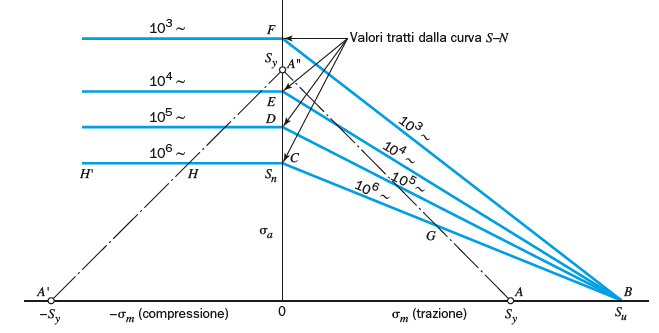
\includegraphics[width=0.5\linewidth]{immagini_11/screenshot008}
				\label{fig:screenshot008}
			\end{figure}
\newpage			
\section{Altre considerazioni sulla curva classica di Wöhler}		
			Tale diagramma viene indicato nei testi anglosassoni come curva SN. 
			\begin{figure}[H]
				\centering
				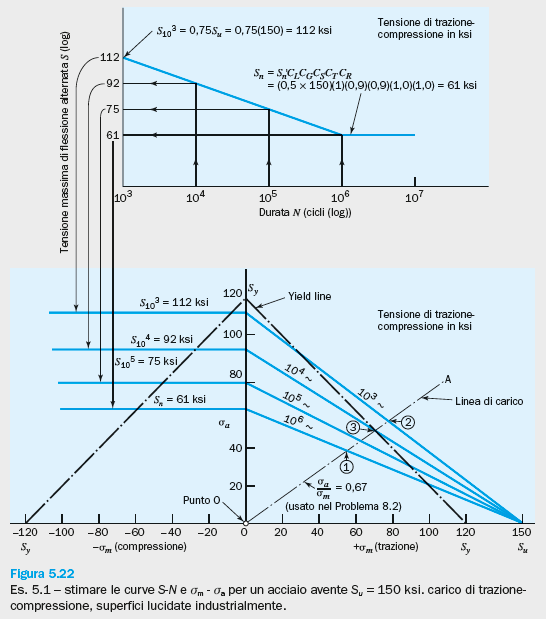
\includegraphics[width=0.5\linewidth]{immagini_11/screenshot009}
				\label{fig:screenshot009}
			\end{figure}
			Per capire quale sia la dipendenza della durata a fatica dalla tensione media qualora non fosse nulla abbiamo bisogno di una diversa rappresentazione, quella di Haig o di Soderberg prevede una diagramma cartesiano in cui la semiampiezza sta in ordinata e la sigma media occupa le ascisse, con dei parametri fissati come il numero di cicli e la probabilità di rottura.
			
			Solitamente si trova che il diagramma di Haig base ha un'affidabilità del 50\% a $20\cdot10^6$ cicli, in quel caso si incontrano sulle ascisse il valore di rottura a semiampiezza nulla e sulle ordinate una tensione media nulla al valore del ginocchio delle curva di Wöhler. 
			
			Dal punto di vista progettuale questa curva è poco pratica, per cui si sono diffusi diagrammi semplificati di Goodman e di Soderberg. 
			
			Un approccio ottimizzato per i materiali duttili, tuttavia, è quello che prevede l'abbinamento del diagramma di Goodman con l'ipotesi che la tensione non debba mai in alcun modo arrivare allo snervamento. Il risultato che si ricava è un'area più ristretta che limita sia a compressione sia a trazione la semiampiezza; a trazione la limitazione (zona esclusa) riguarda alti livelli di tensione media, a compressione invece - se è vero che la fatica non risente del valore assoluto di tensione media di compressione è anche vero che a compressione il materiale non deve assolutamente snervare - si limitano le combinazioni tensione alternata e tensione media. \newline
			
			\textbf{NB:} cosa accade a questo diagramma quando cambio il numero di cicli? 
			
			La costruzione è nata dall'individuare i punti a rottura e snervamento (statici) e con la semiampiezza alternata, che deriva da Wöhler: il ginocchio è il valore di semiampiezza relativo a $2\cdot10^6$ cicli, cambiando il numero di cicli di riferimento basterà porsi su di un diagramma di Wöhler e vedere quale sia il nuovo punto: si osserverà che diminuendo i cicli si aumenta la semiampiezza e questo si traduce nell'imporre un passaggio più in alto sul diagramma corretto, ovvero variare il numero di cicli si traduce in una variazione dell'area sottesa dovuta alla relativa variazione del punto sull'asse delle ordinate. 
			
\newpage			
\section{Goodman-Smith}
			Una rappresentazione alternativa della condizione critica di un materiale a fatica è quella di \textbf{Goodman-Smith}.
\begin{figure}[H]
	\centering
	\label{fig:screenshot010}
	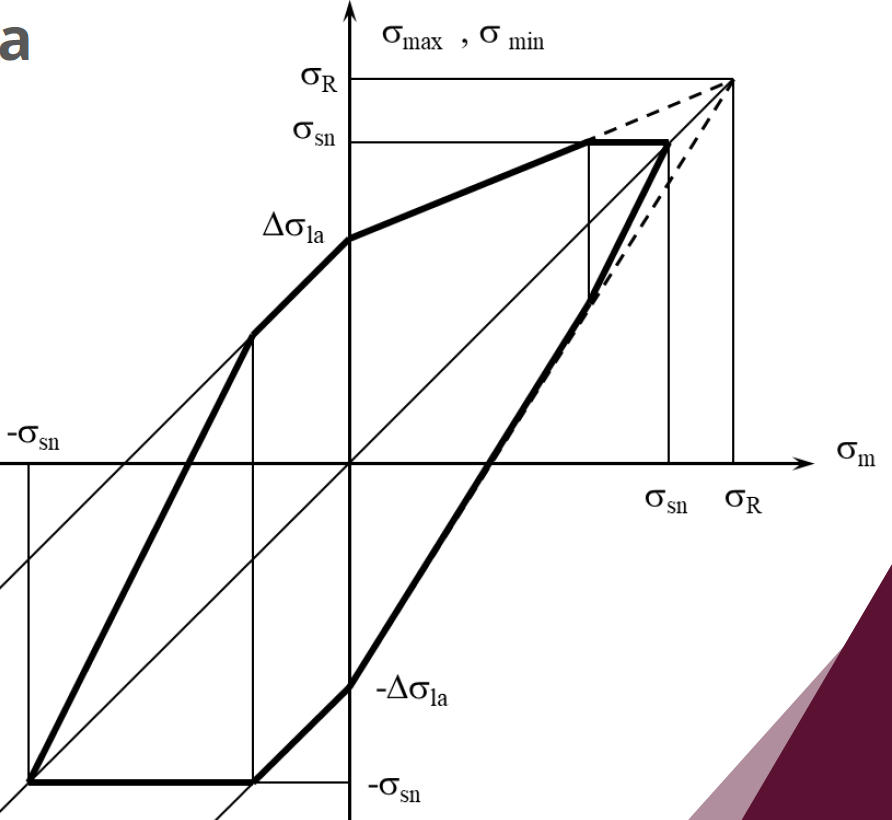
\includegraphics[width=0.5\linewidth]{immagini_11/screenshot010}
\end{figure}			
			Questa rappresentazione utilizza come parametri non semiampiezza e tensione media ma tensione massima e tensione minima, i parametri fissati sono ancora una volta in numero di cicli e la probabilità di rottura. 
			
			In ascissa si trova la tensione media mentre sulle ordinate sono presenti sia il valore massimo che il valore minimo, una curva superiore rappresenta l'andamento della tensione massima ed una curva inferiore quello della minima. \newline
			
			\textbf{Punti caratteristici}
			\begin{enumerate}
				\item \(\sigma_m = 0\) 
				
				Intersezione della curva con l'asse delle $y$, quando la sigma media è nulla  - ipotizzando un numero di cicli pari a quelli del ginocchio di Wöhler - il valore di semiampiezza è noto e pari a $\sigma_{la}$ ed il ciclo sarà esattamente alterno-simmetrico con $R=1$. 
				
				\item \(\sigma_{\max}, \sigma_{min}\)
				
				Poiché il valore massimo è pari al valore minimo in modulo, è possibile individuarle entrambe e poter costruire il diagramma. 
				
				
				\item \textbf{Bisettrice}
				
				La costruzione del diagramma avviene attraverso la bisettrice del primo e terzo quadrante, ovvero quel luogo di punti caratterizzato da coordinate identiche di tensione massima e sigma media.
				
				Cosa significa? 
				
				\begin{itemize}
					\item \(\sigma_{\max} = \sigma_m\)
					
					La sollecitazione è costante e si sta applicando un carico statico: ci si sta muovendo lungo la bisettrice per combinazioni di carico statico ben al di sotto di dei limiti di sicurezza, imposti al massimo per lo snervamento
				\end{itemize}
				
				\item \(\sigma_R\)
				
				La $\sigma_{\max}$, e per costruzione anche la retta per la $\sigma_{\min}$, partono rispettivamente da $\pm\sigma_{la}$ e si raccordano sul vertice a $\sigma_R$. (curva tratteggiata)
				
				\item \textbf{Sollecitazione ciclica}\\
				Si immagini di avere un certo valore di $\sigma_m$ al quale corrispondono un valore di massima ed un valore di minima presi sulle rispettive rette. 
				
				Poiché si è preso un valore di tensione media, questo sarà uguale sia per $x$, che per $y$ (d'altro canto la retta è la bisettrice), per cui la differenza tra le coordinate corrisponde esattamente a $\sigma_m$, questo ci porta a concludere che  la distanza verticale che va dalla retta del massimo alla bisettrice altri non è che la semiampiezza corrispondente a quel tipo di sollecitazione. 
				
				D'altronde la semiampiezza è uguale sia sopra che sotto la sinusoide, proprio per costruzione, allora si è confermato come su questa curva ogni volta che si prende una terna di punti si ha rispettivamente un massimo, una media ed un minimo, ottenendo quest'ultimo imponendo l'uguaglianza delle distanze.
				
				\begin{itemize}
					\item \textbf{Haig}
					
					Il diagramma di Haig utilizzava tensione media e semiampiezza, partiva sulle ordinate da una $\sigma_{la}$ e finiva nel primo quadrante sulle ascisse ad una tensione di rottura, la distanza verticale curva-ascisse era proprio il valore di semiampiezza per un determinato valore di tensione media ed è esattamente la distanza verticale tra la bisettrice e la curva di massimo di Goodman-Smith.
					
					 Se si sceglie un valore di $\sigma_m$ più basso, in Haig ci si avvicina all'asse delle ordinate e la semiampiezza diventava più grande, sempre ricalcando la distanza dalla bisettrice dal valore di massimo di Goodman-Smith. 
					 
					 \item \textbf{Goodman-Smith} 
					 
					 Il diagramma di Goodman-Smith utilizzando massima e minima è "equivalente" al diagramma di Haig ruotato di $45^\circ$ rispetto alla bisettrice: è come se si stesse costruendo il diagramma di Haig sulla bisettrice
					 
				\end{itemize}
				
				\item \textbf{Limitazioni}
				
				La limitazione imposta dai materiali duttili imponeva che la tensione non arrivasse mai allo snervamento, basterà allora limitare superiormente e inferiormente la curva allo snervamento ottenendo una spezzata che limiti le tensioni massime e minime, d'altronde se a parità di tensione media limito la massima sto riducendo la semiampiezza possibile e di conseguenza ho innalzamento della tensione minima: in altre parole, imponendo la limitazione sulla massima si riduce giocoforza la semiampiezza, dato che la minima altro non è che la media meno la semiampiezza, si ottiene un valore di minimo maggiore rispetto a quello che si aveva in precedenza. \newline	
				
				Nella pratica quel ramo di curva (continua, limitata) si ottiene una volta che è stata limitata superiormente la massima a partire dal valore di condizione statica di snervamento, ovvero scendendo giù ed individuando l'ultimo punto valido della vecchia curva: proprio dove si innesta la limitazione.
				
				La minima si sposta sempre in funzione della massima. 
				
				\item \textbf{Compressione} 
				
				Cosa succede dalla parte delle tensioni medie di compressione? 
				
				Il diagramma di Haig proseguiva con semiampiezza costante indipendentemente dal valore di $\sigma_m$.
				
				Nel diagramma di Smith questa semiampiezza è la distanza tra la tensione massima e la bisettrice, significando che il diagramma proseguirebbe con distanza costante. \newline
				
				Poiché il valore di semiampiezza è stato imposto a partire dalle osservazioni sul diagramma Haig, lo stesso si può fare anche per la tensione minima: se $\sigma_{\max} - \sigma_m$ forniscono la distanza per le tensioni di trazione, allora lo stesso varrà, con uguale valore, anche per la compressione e $\sigma_m-\sigma_{\min}$ fornirà la distanza per le tensioni di compressione. 
				
				L'andamento della minima passa per le -$\sigma_{la}$ ed è parallelo alla bisettrice. \newline
				
				Imponendo un limite allo snervamento (o alla rottura) si va a limitare il valore della tensione minima, questa altri non è che la minima algebrica può al più esser pari allo snervamento.
				
				Come fatto per la trazione si procede limitando la minima con lo snervamento, ora che si è notevolmente ridotto il valore di semiampiezza, questo valore sommato alla media individua la massima: il nuovo punto proiezione. Ripetendo il ragionamento della trazione si ottiene il nuovo ramo di curva di tensione massima.
											
			\end{enumerate}
			
			Questa tuttavia rimane una costruzione semplificata: con tutte queste spezzate non si fa altro che rincorrere i dati sperimentali.  
			
			Il diagramma così riportato è tipico dei materiali duttili.
			
			Tutto ciò questo è stato tuttavia tracciato per un numero di cicli prefissato, come quello del ginocchio di Wöhler. 
			
			Qualora fossi di fronte ad un numero di cicli differente da quello di Wöhler, significherebbe avere:
				\begin{itemize}
				\item Per un numero di cicli inferiore un diagramma che si amplierebbe similmente ad un diagramma di Haig. 
				
				Infatti se passo ad un numero di cicli inferiore, si aumenta il valore di semiampiezza e l'intercetta $\sigma_{la}$ sale di quota;
				
				\item Per un un numero di cicli superiore si assottiglierebbe, avvicinandosi le le intercette sull'asse delle y. 
				
			\end{itemize} 
			

\subsection{Master Diagram	}					
			In questa rappresentazione si rapportano nelle due coordinate i valori di $\sigma_{\max}$ e $\sigma_{\min}$ e si diagrammano gli andamenti nelle due bisettrici. 
				
			Quando massimo e minimo sono uguali tra loro $R=1$ e allora siamo in condizioni statiche, quando siamo sull'altra bisettrice $R=-1$ e la minima è uguale alla massima in modulo ma opposta in segno e siamo in condizioni alterno simmetrica.
			\begin{figure}[H]
				\begin{subfigure}{0.5\textwidth}
					\centering
				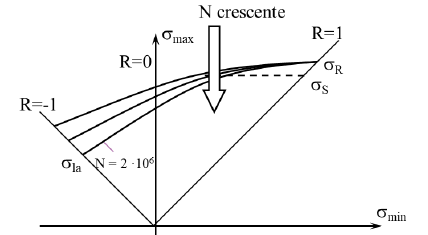
\includegraphics[width=0.9\linewidth]{immagini_11/screenshot011}
				\end{subfigure}%
				\begin{subfigure}{0.5\textwidth}
					\centering
				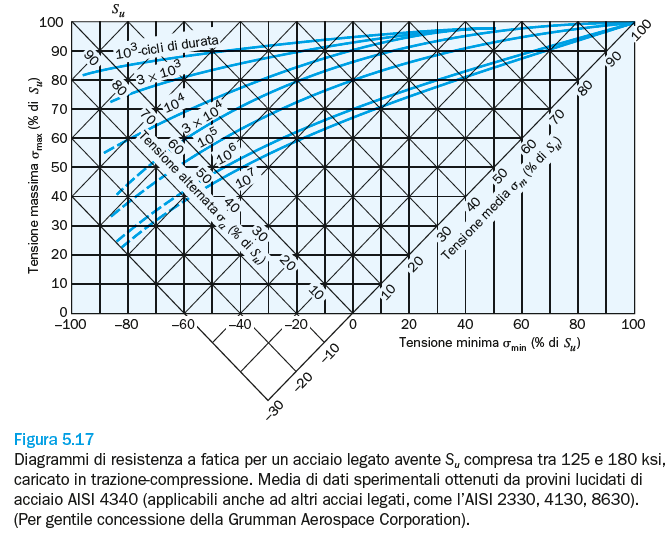
\includegraphics[width=0.9\linewidth]{immagini_11/screenshot012}
				\end{subfigure}
			\end{figure}
			
\section{Stati di tensioni non monodimensionali	}					
			
			Il caso più comune è quello dell'albero di trasmissione. 
			
			Questo organo meccanico è soggetto a flessione rotante e a momento torcente. 
			
			Il momento flettente è costante nel tempo ma siccome l'albero ruota la tensione è variabile sinusoidalmente nel tempo: questa altri non è che la componente $\sigma_z$ del tensore delle tensioni.
			
			Il momento torcente sarà invece costante nel tempo: è necessario trasmettere momento torcente continuativamente. Questa sollecitazione è identificata dalle componenti $\tau_z$ del tensore delle tensioni. \newline
			
			Come si procede in questo studio? Solitamente si utilizzano delle formulazioni che si basano su criteri di resistenza statici come magari Von Mises, solo che siccome sono sollecitazioni diverse tra loro come tipologia e formulazioni, attualmente si preferisce, anziché confrontare la combinazione delle tensioni con una tensione limite, normalizzare le tensioni per il proprio limite.
			\[\sigma_{id} = \sqrt{\sigma^2 + 4\tau^2} \qquad \text{Ip. Max tensione tangenziale}\]
			\[\sigma_{id} = \sqrt{\sigma^2 + 3\tau^2} \qquad \text{Ip. Von Mises o Max energia di distorsione tangenziale}\]
			\[\sigma_{id} = \sqrt{\sigma^2 + \alpha^2\tau^2} \qquad \text{Ip. generica} \qquad \alpha = \dfrac{\sigma_{lim}}{\tau_{lim}}\]

			Questo vuol dire che la tensione limite per le $\sigma$, se questa è variabile nel tempo, sarà un limite di fatica, mentre quella sulle $\tau$ se questa è costante nel tempo, sarà un limite statico.
			
			Se addirittura si hanno tensioni in due direzioni (caso $xy$) allora si può utilizzare la relazione di Von Mises in cui la normalizzazione anziché essere fatta tramite lo stesso limite viene effettuata con limiti distinti, separati, ciascuno per la tipologia di sollecitazione presente. 
			
			Lo sviluppo di questo studio è dovuto a Gaugh e Pollard ed è nato proprio dall'analisi degli alberi di trasmissione.
			
			Senza scendere troppo nel dettaglio, in un piano cartesiano $\sigma\tau$, il limite è dettato da una curva che può essere approssimata come arco d'ellisse o come quarto di ellisse. 
\begin{figure}[H]
	\centering
	\label{fig:screenshot013}
	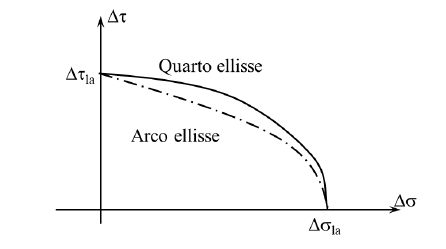
\includegraphics[width=0.5\linewidth]{immagini_11/screenshot013}
\end{figure}			
			Le normative utilizzano sostanzialmente il quarto d'ellisse. 
			
			In queste formulazioni:
			\[\left(\dfrac{\sigma}{\sigma_{lim}}\right)^2 + \left(\dfrac{\tau}{\tau_{lim}}\right)^2\leq1 \qquad \text{Monodimensionale + torsione/taglio}\]
			
			\[\left(\dfrac{\sigma_x}{\sigma_{x,lim}}\right)^2 + \left(\dfrac{\sigma_y}{\sigma_{y,lim}}\right)^2 - \dfrac{\sigma_x\sigma_y}{\sigma_{x,lim}\sigma_{y,lim}} + \left(\dfrac{\tau}{\tau_{lim}}\right)^2\leq1 \qquad \text{Bidimensionale + torsione/taglio}\]
			Ciascuna componente del tensore è separata e normalizzata rispetto a proprio limite. \newpage
			
\section{Progettazione a fatica}						
			Quando si tratta la progettazione in ambito di fatica devo necessariamente tenere conto di un elemento: l'affidabilità. 
			
			Ogni dato sperimentale di fatica dev'essere interpretato con una distribuzione come quella gaussiana.
			
			Ad una distribuzione di punti sperimentali si associano le curve di Wöhler di tendenza per una probabilità di rottura del 10, 50 e 90\%. 
\begin{figure}[H]
	\centering
	\label{fig:screenshot014}
	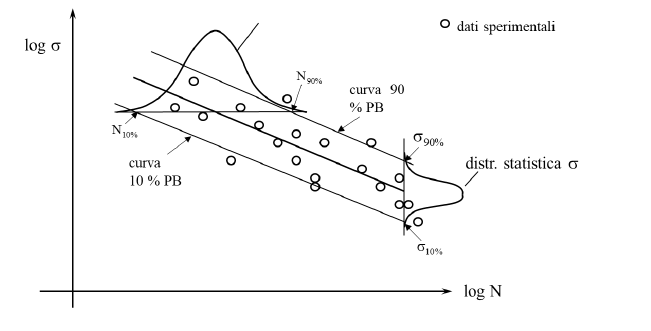
\includegraphics[width=0.7\linewidth]{immagini_11/screenshot014}
\end{figure}
			\textbf{PB}: Rottura, \textbf{PR}: Reliability
			
			Fissato un certo numero di cicli, leggo nei dati sperimentali un certo livello di tensione al quale è associata una probabilità di sopravvivenza del 90\% e un certo dato di tensione per cui è associata una probabilità di sopravvivenza del 10\%; al contrario un valore a cui è associato un 10\% di rottura è uno a cui è associato il 90\% di probabilità di rottura: la distribuzione statistica rispetto alle tensioni è piuttosto stretta. \newline 
			
			Tuttavia se si considera un determinato livello di carico, ad un valore del numero di cicli a cui è associato un 10\% di rottura (o 90\% di sopravvivenza) si individua un valore molto diverso da quello a cui è associato il 90\% di rottura o 10\% di sopravvivenza per cicli fissati: vuol dire che la distribuzione statistica dei dati sperimentali a partirà di tensione (e quindi rispetto al numero di cicli) è decisamente più ampia, i dati sono molto più distribuiti, e l'incertezza sul valore di durata di un componente fissata la tensione è molto più elevata rispetto all'incertezza sul valore di tensione a numero di cicli fissato.  
			
			Come si fa nella pratica realizzativa? 
			
			Si usano vari diagrammi sperimentali.		
			Curve semi-logaritmiche, diagrammi sperimentali,...

\section{Coefficiente di sicurezza in fatica}
			Il fattore di sicurezza come si ricava? 
			
			Come il rapporto tra la tensione massima che si potrebbe avere a quel livello di carico (a un certo numero di cicli) rispetto alla tensione effettiva a quel livello di carico a quel numero di cicli.  
			\begin{figure}[H]
				\centering
				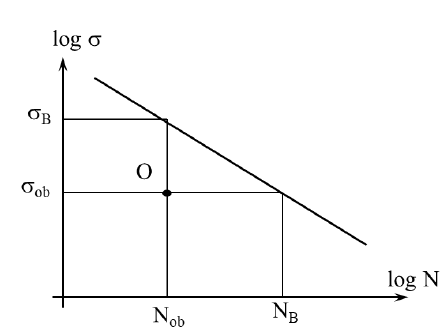
\includegraphics[width=0.4\linewidth]{immagini_11/screenshot018}
				\label{fig:screenshot018}
			\end{figure}			
			Se ho il punto di lavoro O caratterizzato da una $\sigma_O$ ed $N_O$, il fattore di sicurezza è il rapporto fra la tensione/semiampiezza massima che porrei avere a quel numero di cicli di applicazione rispetto a quella che sto applicando; mentre il fattore di sicurezza sul numero di cicli è il rapporto fra il numero massimo di cicli che potrei avere a quel livello di carico, rispetto al numero di cicli effettivamente applicato, ora questi punti massimi $\sigma_B$ ed $N_B$ sono in relazione fra loro con la legge di Wöhler per cui:
			\[\gamma_\sigma = \dfrac{\sigma_B}{\sigma_{ob}} \qquad \gamma_N = \dfrac{N_B}{N_{ob}} \qquad \gamma_N>\gamma\sigma\]
			\[N_{ob}\sigma_B^k = N_B\sigma_{ob}^k\]
			\[\gamma_N=\gamma_\sigma^k\]			
			Ora se si sceglie convenzionalmente un fattore di sicurezza pari a 1,6 sulle tensioni - ricordando che il coefficiente $k$ a seconda di come è fatto il provino può variare tra 3 e 10 - si ottiene che a pari affidabilità il fattore di sicurezza sul numero di cicli $\gamma_N$ varia tra 4 e 100, potendo imporre un numero di cicli a pari affidabilità di due ordini di grandezza inferiore rispetto a quelli limite mantenendo la stessa sicurezza. 
			
\section{Curva SN per sollecitazione media non nulla}
			Avendo visto i diagrammi di fatica più comuni si è ora in grado di quantificare come impatta un valore di tensione media non nulla sul diagramma di Wöhler. \newline
			
			Come possiamo correggere il diagramma di Wöhler standard e trasformarlo nel diagramma di Wöhler per l'applicazione specifica?
			
			Per far questo è necessario iniziare a tracciare il diagramma di Haig standard per $10^6$ cicli, com'è noto si costruisce utilizzando il ginocchio di Wöhler sulle $y$ e la rottura sulle $x$ limitando il diagramma con lo snervamento ottenendo quindi un altro diagramma standard. 
\begin{figure}[H]
	\centering
	\label{fig:screenshot019}
	
\includegraphics[width=0.5\linewidth]{immagini_11/screenshot019}
\end{figure}
			Qualora in ginocchio di Wöhler non fosse disponibile da tabelle specifiche si può prendere per materiali duttili comuni il valore della $\sigma_{la}$ come il 30$\div$50\% della rottura. 
			\[\text{fattore di fatica}\,=\dfrac{\sigma_{la}}{\sigma_R}\] 						
			Siccome si vuole tracciare il diagramma di Haig e Wöhler per il pezzo specifico con $\sigma_m\ne0$ si corregge il diagramma anche in funzione di tutti quei coefficienti che spostano il ginocchio.
			
			A seconda di quale sia il livello di scostamento dalla condizione standard, riducendo la semiampiezza effettiva si otterrà la $\sigma_{la-effettiva}$: per il limite di fatica effettivo si partirà comunque dal limite a fatica del materiale per cui il diagramma si sposterà più in basso. \newline 
			
			A questo punto è possibile ricavare il nuovo valore del ginocchio della curva di Wöhler: sia per ipotesi $\sigma_m = sigma_m^*$ di trazione (sempre per $10^6$ cicli), il nuovo ginocchio si andrà a cercare per il $\sigma_m^*$ desiderato, il punto di intersezione così individuato darà alla luce anche il nuovo valore $\sigma_{la}^*$ del ginocchio di Wöhler relativamente alla $sigma_m^*$ di input del problema, ecco allora come si è ridefinito il punto G del ginocchio.
			\begin{figure}[H]
				\centering
				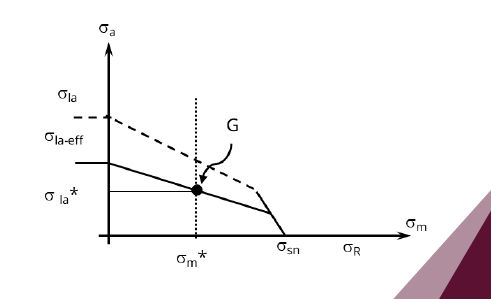
\includegraphics[width=0.5\linewidth]{immagini_11/screenshot020}
				\label{fig:screenshot020}
			\end{figure}			 						
			Siccome però la rappresentazione di Wöhler è data dal numero di cicli rispetto alla semiampiezza di sollecitazione, si deve ragionare anche sul punto S, il punto di confine con quella che sarà poi la fatica oligociclica.
			\begin{figure}[H]
				\centering
				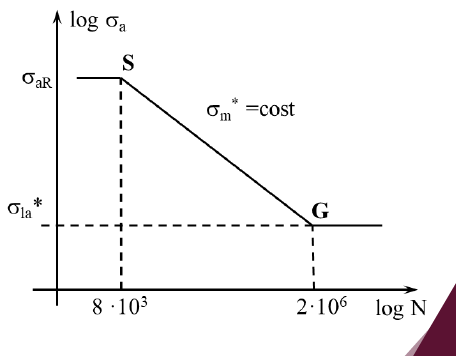
\includegraphics[width=0.5\linewidth]{immagini_11/screenshot021}
				\label{fig:screenshot021}
			\end{figure}			
			 Le vecchie coordinate di quel valore erano $8\cdot10^3$ cicli con sigma di rottura data nel caso di sigma media nulla: il punto S corrisponde ad uno spettro di sollecitazione nel tempo sinusoidale, perfettamente simmetrico dove il valore massimo era la sigma di rottura. 
			 
			 Poiché devo rappresentare la semiampiezza, questa per $\sigma_m=0$ era esattamente la massima, la rottura, nel momento in cui la $\sigma_m\ne0$, il mio ciclo trasla verso l'alto sempre limitato superiormente dalla rottura e quindi S rappresenta la condizione di carico in cui la massima ha raggiunto la rottura: in queste condizioni la semiampiezza varrà $\sigma_{aR} = \sigma{R} -\sigma_m$, questa nuova semiampiezza caratterizza così lo spettro di carico del punto S. In questo punto l'abbassamento è semplicemente dovuto alla $\sigma_m$ e non dipende da nient'altro; l'abbassamento del ginocchio è invece funzione dei coefficienti correttivi e dello spostamento della curva di Haig da $\sigma_{la}$ a $\sigma_{la-effettiva}$: è molto più complesso il meccanismo che ha portato a spostare il ginocchio che quello che ha spostato il punto S. \newline
						
			Si può ripetere lo steso ragionamento qualora anziché correggere il diagramma di Wöhler con una $\sigma_m\ne0$, volessi correggere il diagramma di Wöhler perché ho un diverso rapporto di ciclo $R$. 
			
			Il ragionamento è praticamente il medesimo: si riduce il diagramma di Haig ad uno effettivo di Haig considerando i coefficienti di correzione, gli aspetti interni ed esterni del componente e a quel punto anziché imporre una sigma media individuo la retta corrispondente al rapporto di ciclo desiderato, l'intersezione darà il nuovo ginocchio di Wöhler e di conseguenza diviene possibile correggere il resto.

		\begin{figure}[H]
		\includegraphics[scale=0.75,page=21]{11_fcm_2022}
		\end{figure}
